\section{Web Interface}

The web interface is a simple web application that allows users to interact with the system.
It allows users to execute the 5 operations previously described. 
\subsection{Backend}
It is implemented using the Flask web framework of Python.

\begin{lstlisting}
    # app.py
from flask import Flask, render_template, request, redirect, url_for, flash
import oracledb
import datetime

app = Flask(__name__)
app.secret_key = 'supersecretkey'  # per flash messages

# Configurations parameters for the Oracle DB
DB_USER = 'System'
DB_PASSWORD = 'password123'
DB_SID = 'localhost:1521/xe'


def get_db_connection():
    try:
        connection = oracledb.connect(user=DB_USER, password=DB_PASSWORD, dsn=DB_SID)
        return connection
    except Exception as e:
        print("Errore nella connessione al DB:", e)
        return None

# Homepage
@app.route('/')
def index():
    return render_template('index.html')

# Operation 1: Register a new customer
@app.route('/register_customer', methods=['GET', 'POST'])
def register_customer():
    if request.method == 'POST':
        code = request.form.get('code')
        name = request.form.get('name')
        surname = request.form.get('surname')
        email = request.form.get('email')
        cust_type = request.form.get('cust_type')
        dob_str = request.form.get('dob')
        try:
            dob = datetime.datetime.strptime(dob_str, '%Y-%m-%d').date()
        except Exception as e:
            flash("Birth date non valida", "danger")
            return redirect(url_for('register_customer'))

        conn = get_db_connection()
        if conn is None:
            flash("Connection error", "danger")
            return redirect(url_for('register_customer'))
        try:
            cur = conn.cursor()       
            cur.callproc("proc_register_customer", [code, name, surname, email, cust_type, dob])
            conn.commit()
            flash("Customer added successfully", "success")
        except oracledb.DatabaseError as e:
            flash(f"Error during customer registration: {e}", "danger")
        finally:
            cur.close()
            conn.close()
        return redirect(url_for('index'))
    return render_template('register_customer.html')

# Operation 2: Add a new energy contract
@app.route('/add_contract', methods=['GET', 'POST'])
def add_contract():
    if request.method == 'POST':
        contract_id = request.form.get('contract_id')
        contract_type = request.form.get('contract_type')
        start_date_str = request.form.get('start_date')
        energy_plan = float(request.form.get('energy_plan'))
        duration = float(request.form.get('duration'))
        account_code = request.form.get('account_code')
        facility_name = request.form.get('facility_name')
        try:
            start_date = datetime.datetime.strptime(start_date_str, '%Y-%m-%d').date()
        except Exception as e:
            flash("Not a valid date", "danger")
            return redirect(url_for('add_contract'))

        conn = get_db_connection()
        if conn is None:
            flash("Error during connection to the database", "danger")
            return redirect(url_for('add_contract'))
        try:
            cur = conn.cursor()
           
            cur.callproc("proc_add_contract", [contract_id, contract_type,
                                                 start_date, energy_plan, duration,
                                                 account_code, facility_name])
            conn.commit()
            flash("Contract added successfully", "success")
        except Exception as e:
            flash(f"Error during contract addition: {e}", "danger")
        finally:
            cur.close()
            conn.close()
        return redirect(url_for('index'))
    return render_template('add_contract.html')

# Operation 3: Assign a facility to a management team
@app.route('/assign_facility', methods=['GET', 'POST'])
def assign_facility():
    if request.method == 'POST':
        facility_name = request.form.get('facility_name')
        team_code = request.form.get('team_code')
        conn = get_db_connection()
        if conn is None:
            flash("Error during connection to the database", "danger")
            return redirect(url_for('assign_facility'))
        try:
            cur = conn.cursor()
            cur.callproc("proc_assign_facility", [facility_name, team_code])
            conn.commit()
            flash("Facility assigned successfully", "success")
        except Exception as e:
            flash(f"Error during facility assignment: {e}", "danger")
        finally:
            cur.close()
            conn.close()
        return redirect(url_for('index'))
    return render_template('assign_facility.html')

# Operation 4: View the total energy output of a facility managed by the eldest employee
@app.route('/view_facility_energy', methods=['GET', 'POST'])
def view_facility_energy():
    facilities = []
    energy_output = None

    # 1. Query to retrieve the oldest manager's team code
    conn = get_db_connection()
    if conn is None:
        flash("Error during connection to the database", "danger")
        return redirect(url_for('index'))
    try:
        cur = conn.cursor()
        query_oldest_manager = """
            SELECT DEREF(e.Team).Code AS team_code
              FROM Employee e
             WHERE e.Manager = 'Y'
             AND e.Team IS NOT NULL
             ORDER BY e.DoB ASC
             FETCH FIRST 1 ROWS ONLY
        """
        cur.execute(query_oldest_manager)
        result = cur.fetchone()
        if result is None:
            flash("No manager found", "danger")
        else:
            team_code = result[0]
            # 2. Query to retrieve the facilities managed by the oldest manager
            query_facilities = """
                SELECT f.Name 
                  FROM Facility f
                 WHERE DEREF(f.Team).Code = :team_code
            """
            cur.execute(query_facilities, {'team_code': team_code})
            facilities = [row[0] for row in cur.fetchall()]
    except Exception as e:
        flash(f"Error during data retrieval: {e}", "danger")
    finally:
        cur.close()
        conn.close()

    # 3. Retrieve the total energy output of the selected facility
    if request.method == 'POST':
        selected_facility = request.form.get('facility')
        conn = get_db_connection()
        if conn is None:
            flash("Error during connection to the database", "danger")
            return redirect(url_for('view_facility_energy'))
        try:
            cur = conn.cursor()
            # Chiamata alla funzione SQL per ottenere il totale dell'energia in output
            energy_output = cur.callfunc("func_get_facility_energy", oracledb.NUMBER, [selected_facility])
            flash(f"Total Energy Output for {selected_facility}: {energy_output}", "success")
        except Exception as e:
            flash(f"Error during data retrieval: {e}", "danger")
        finally:
            cur.close()
            conn.close()

    return render_template("view_facility_energy.html", facilities=facilities, energy_output=energy_output)

# Operation 5: Print a ranked list of facilities based on their efficiency scores
@app.route('/ranked_facilities')
def ranked_facilities():
    facilities = []
    conn = get_db_connection()
    if conn is None:
        flash("Errore di connessione al database", "danger")
        return redirect(url_for('index'))
    try:
        cur = conn.cursor()
        out_cursor = cur.var(oracledb.CURSOR)
        cur.callproc("proc_get_ranked_facilities", [out_cursor])
        result_cursor = out_cursor.getvalue()
        facilities = result_cursor.fetchall()
    except Exception as e:
        flash(f"Errore durante il recupero dei dati: {e}", "danger")
    finally:
        cur.close()
        conn.close()
    return render_template('ranked_facilities.html', facilities=facilities)

if __name__ == '__main__':
    app.run(debug=True)
\end{lstlisting}

\subsection{Frontend}

\begin{figure}[H]
    \centering
    \includegraphics[width=\textwidth]{images/homepage.png}
    \caption{Homepage}
\end{figure}

\begin{figure}[H]
    \centering
    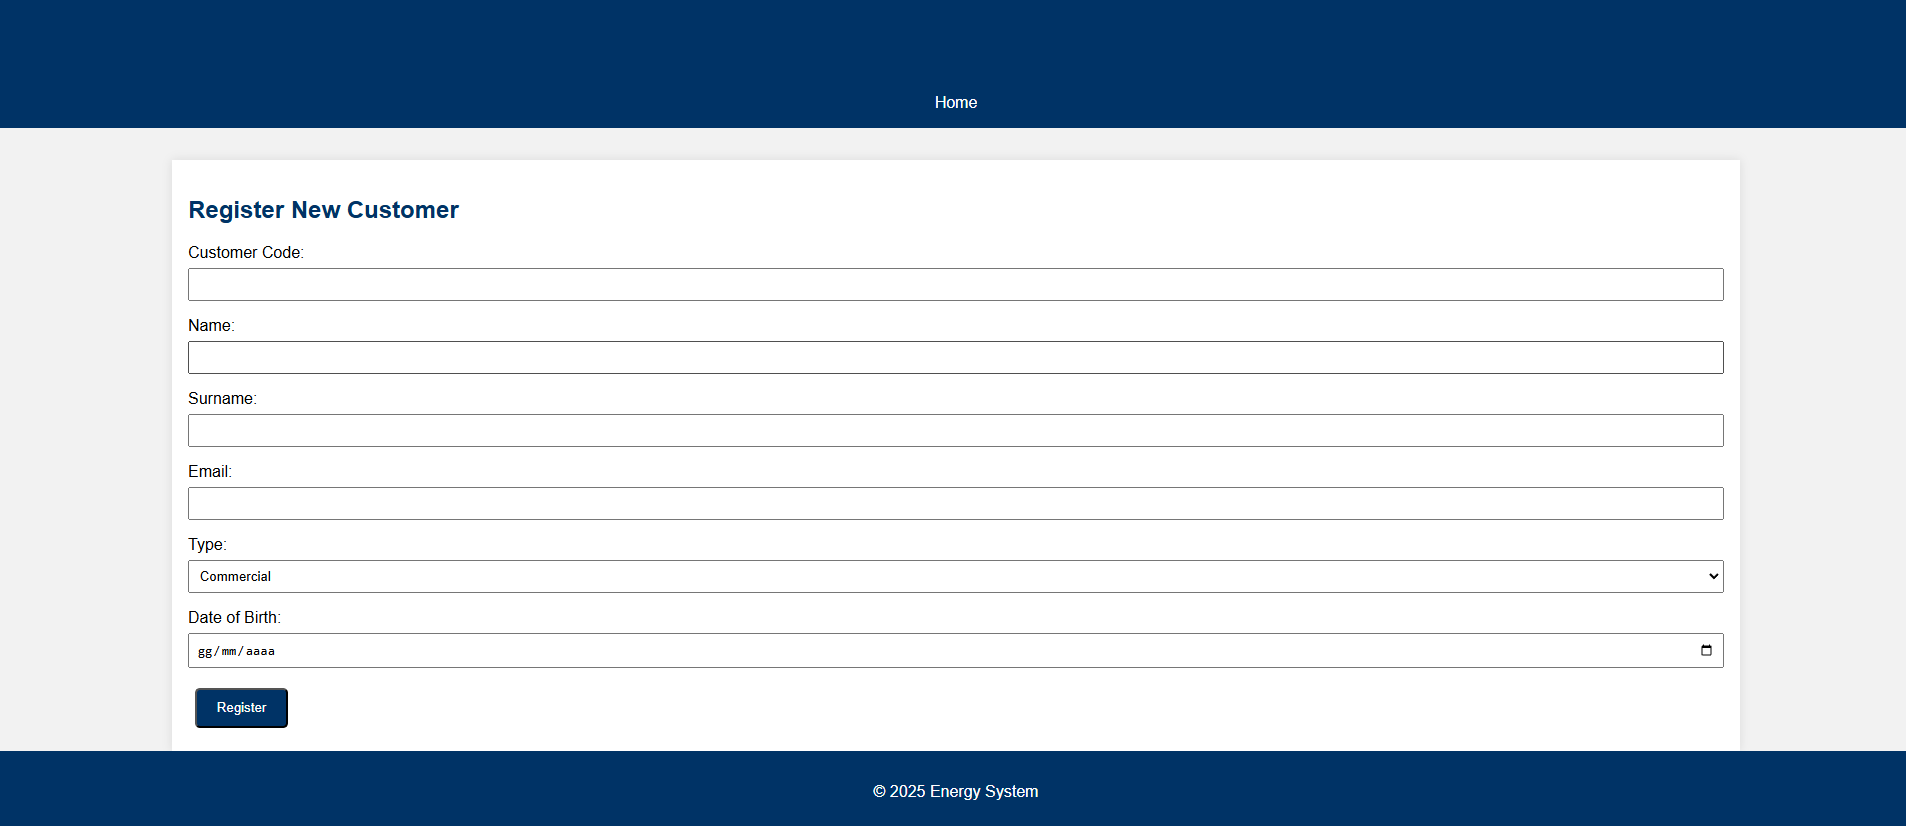
\includegraphics[width=\textwidth]{images/Op1.png}
    \caption{Register a new customer}
\end{figure}


\begin{figure}[H]
    \centering
    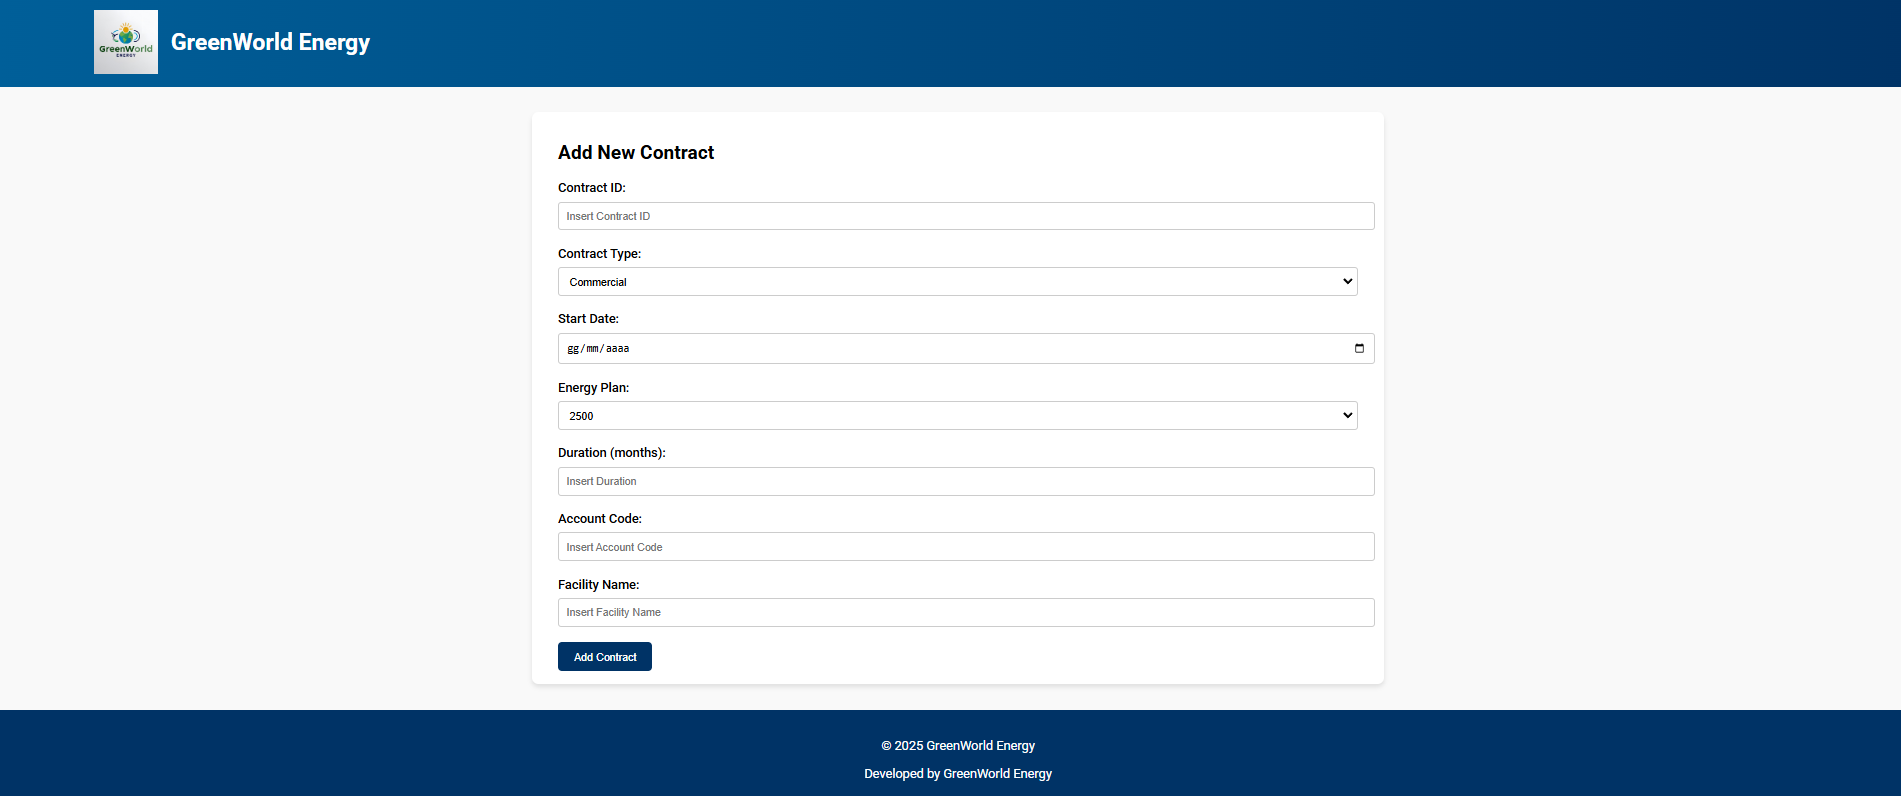
\includegraphics[width=\textwidth]{images/Op2.png}
    \caption{Add a new energy contract}
\end{figure}


\begin{figure}[H]
    \centering
    
\includegraphics[width=\textwidth]{images/Op3.png}
    \caption{Assign a facility to a management team}
\end{figure}


\begin{figure}[H]
    \centering
    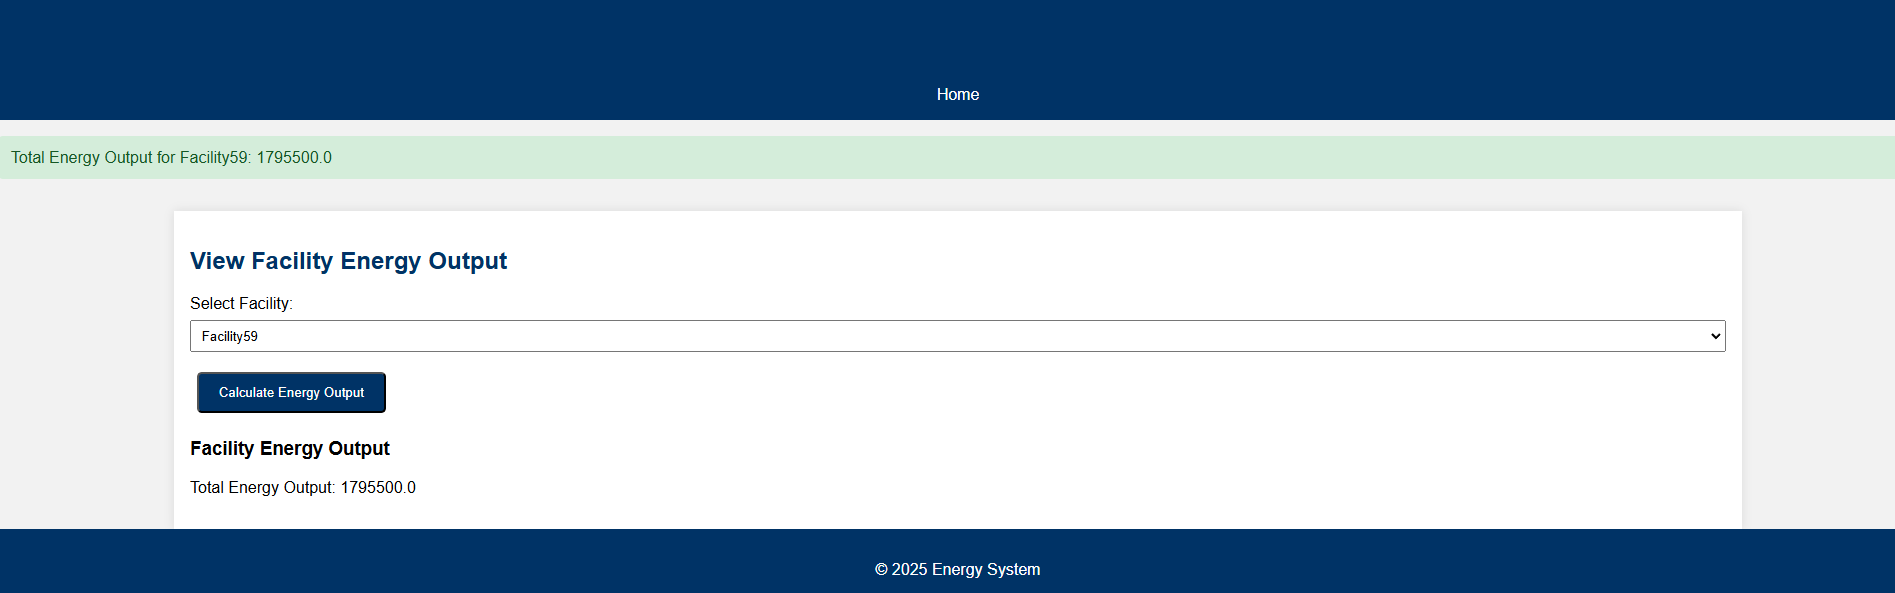
\includegraphics[width=\textwidth]{images/Op4.png}
    \caption{View the total energy output of a facility managed by the eldest employee}
\end{figure}


\begin{figure}[H]
    \centering
    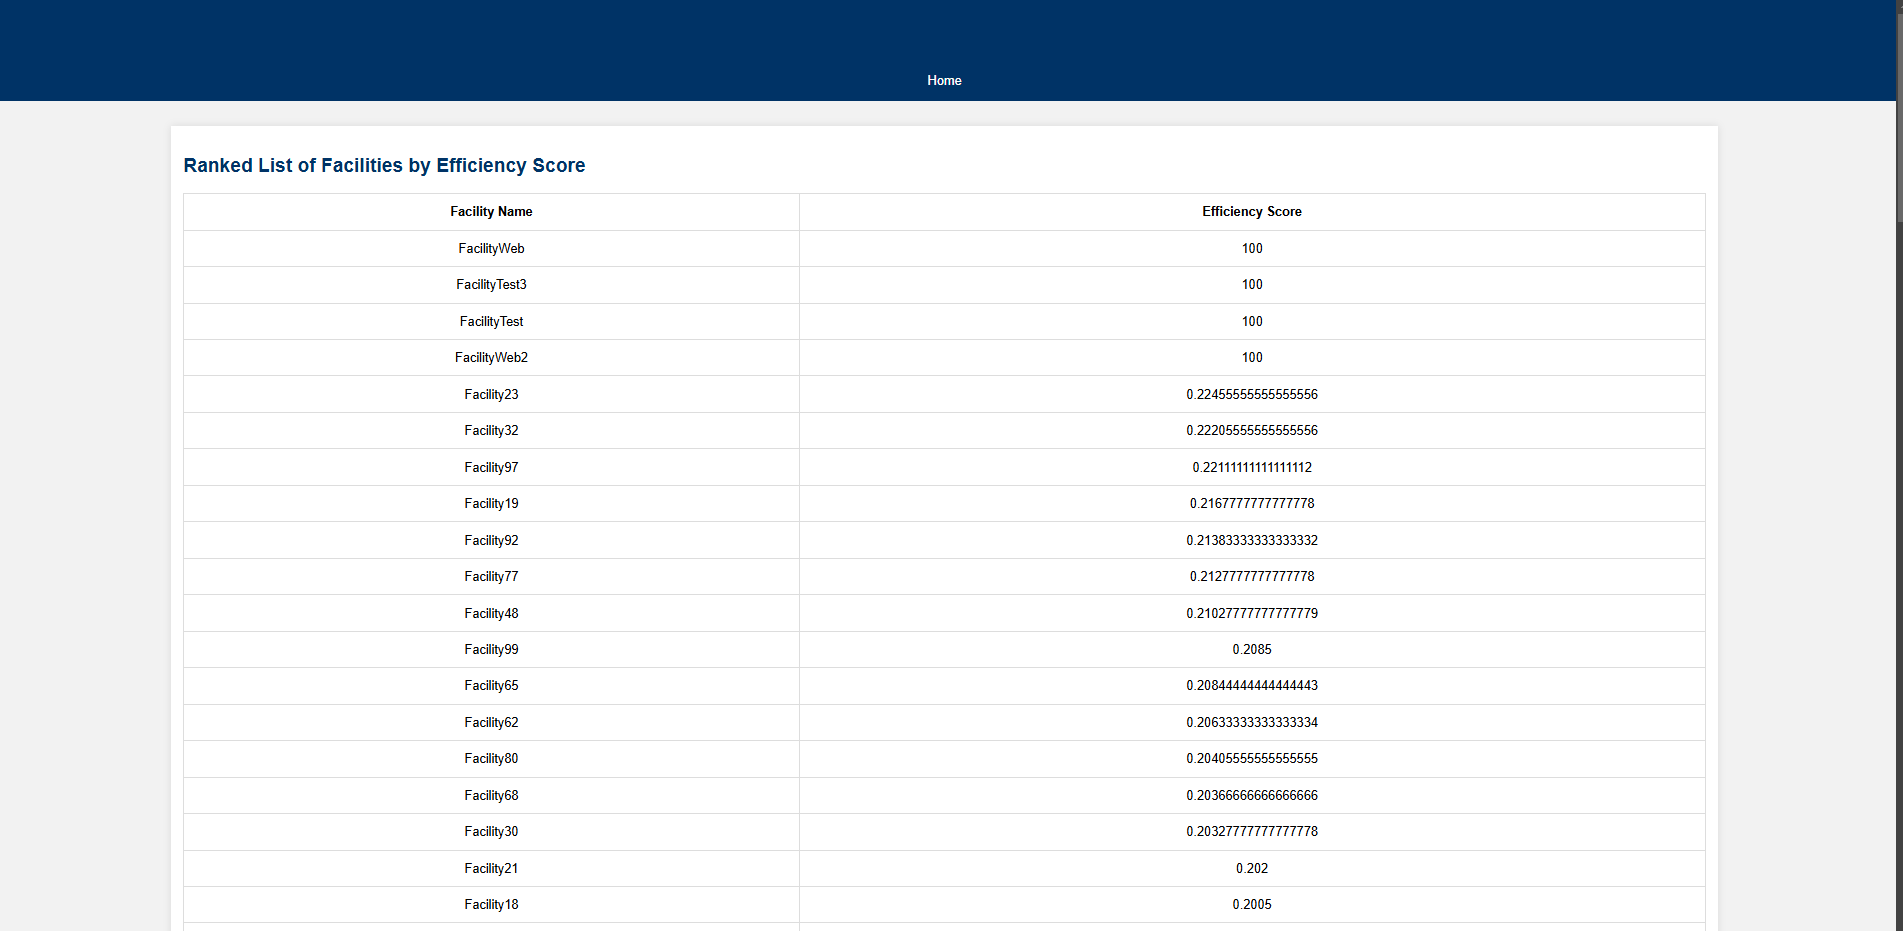
\includegraphics[width=\textwidth]{images/Op5.png}
    \caption{Print a ranked list of facilities based on their efficiency scores}
\end{figure}